\documentclass{ReportCUNY}
\usepackage{array}
\usepackage{xspace}

\AssetPath{data/}
\CourseName{Distributed and Cloud Computing}
\CourseNumber{85011}
\CitationFile{./data/references.bib}
\DateD{31}
\DateM{10}
\DateY{2022}
\DepartmentAbbrev{CSc}
\DepartmentName{Computer Science}
\Institution{The Graduate Center~--~CUNY}
\Instructor{Saptarshi Debroy}
\Student{Isa Jafarov, Nan Jia, Alex Washburn, Rose Wong}
\Subtitle{STREAM: Course Project Plan}
\Title{Simple \& Transparent Resource\\\vspace*{-8mm}Exchange And Management}

\newcommand{\Nat}{\ensuremath{\mathbb{N}}\xspace}
\newcommand{\PosInt}{\ensuremath{\mathbb{Z}^{+}}\xspace}
\newcommand{\KeyWord}[1]{\textbf{\texttt{#1}}}
\newcommand{\KeyValuePair}[2]{\KeyWord{#1}\;:\qquad#2}
\newcommand{\KeyTypeValuePair}[3]{\KeyWord{#1}:~\makebox[2cm][l]{#2}~\qquad#3}
\newcommand{\WorkloadStudentTaksPair}[2]{\makebox[2.75cm][l]{#1:}~#2}

\newcommand{\MonthDayFormat}[2]{\textbf{\texttt{#1}}~--~\textbf{\texttt{#2}}}

\begin{document}
\setlength{\belowdisplayskip}{0pt} \setlength{\belowdisplayshortskip}{1pt}
\setlength{\abovedisplayskip}{0pt} \setlength{\abovedisplayshortskip}{1pt}
\setlength{\abovedisplayskip}{5pt}
\setlength{\belowdisplayskip}{5pt}

\section{Introduction}

The course project comprises the creation of a distributed ``Science Broker'' which manages requests for scientific resources and information.
We will fulfill the project requirements by designing and implementation a service which receives requests for resources to satisfy a scientific job submission.
Furthermore, the service will be implemented in a distributed manner, permitting the sharing of resources across collaborating scientific ``domains.''


\section{Design}

\subsection{Overview: Utilize GENI multi-cloud topology}

We will use GENI to simulate multiple collaborating scientific institutions.
Each scientific organization will form a \KeyWord{Domain}.
A \KeyWord{Domain} is a network topology of resources contained entirely within a ``real'' GENI site.
Multiple \KeyWord{Domain} will be connected together within GENI to form a multi-cloud topology.
Every \ \KeyWord{Domain} has an \KeyWord{Endpoint} facilitating \KeyWord{User} access to the entire multi-cloud topology which comprises the Science Broker Service.
A \KeyWord{User} can submit a \KeyWord{Job} through an \KeyWord{Endpoint} by specifying the required resources.

Furthermore there will be an additional \KeyWord{Domain} containing containing the \KeyWord{Broker}.
All resources across all \KeyWord{Domain}s are known to the \KeyWord{Broker}.
Hence, the \KeyWord{Broker} handles scheduling, networking, and load balancing of submitted \KeyWord{Job}s.


\subsection{Broker}

The \KeyWord{Broker} agent/instance is the centralized manager of the Science Broker Service.
Encapsulated within the \KeyWord{Broker} is the maintenance of an ACID database containing:
\begin{itemize}
\item A list of all incomplete \KeyWord{Job} submissions.
\item A list of all resources across each \KeyWord{Domain}.
\item A mapping of which resource(s) are allocated to which \KeyWord{Job}.
\item A queue of pending \KeyWord{Job} submissions.
\end{itemize}

Additionally, the \KeyWord{Broker} executes a scheduling algorithm to determine which queued \KeyWord{Job} will be given which resource(s) and when a \KeyWord{Job} will be migrated.

\begin{figure}
	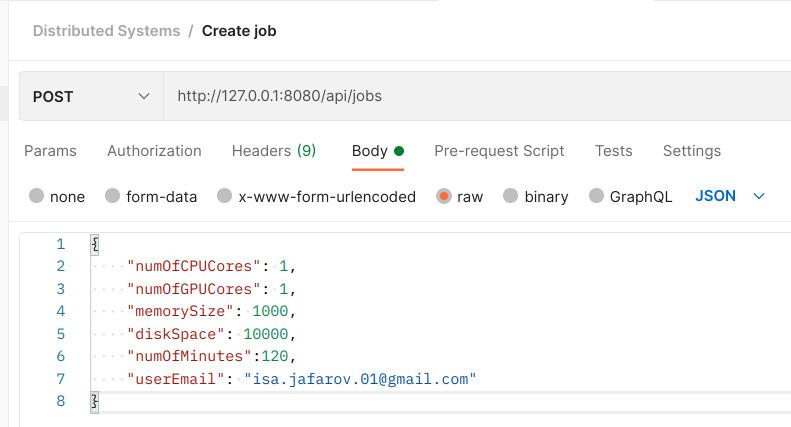
\includegraphics[width=\textwidth]{Backend-API-Demo.jpeg}
	\caption{Example request received by ``Back-end''  \KeyWord{Broker}.}
\end{figure}


\subsection{Scheduling \& Queuing}

Testing possible scheduling algorithms that are:
\begin{itemize}
\item FCFS(first come first serve)
\item SJF(shortest job first)
\item RR(round robin)
\end{itemize}

Because we focus on monitoring our brokering network's resource management and performance. Those three algorithms have different advantages and disadvantages. 


\subsection{Domains}

Within the multi-cloud topology, there are many \KeyWord{Domain}s.
Each \KeyWord{Domain} contributes one or more computing resources to the multi-cloud topology.
Additionally, each \KeyWord{Domain} locally hosts an \KeyWord{Endpoint} from which a \KeyWord{User} within the \KeyWord{Domain} can access the computing resources of the science brokering service by submitting a \KeyWord{Job}.
Networked communication and computations across domains are dynamically mediated by the \KeyWord{Broker}.


\subsection{Replication}

We will use Docker containers and Kubernetes to manage workload distribution, backup, and migration.
This will make it easier for us to manage and scale the science brokering service.


\subsection{Jobs}

A \KeyWord{Job} contains the following information:

\begin{itemize}
\item \KeyTypeValuePair{Mail}{String}{An email address for the user, uniquely identifies user}
\item \KeyTypeValuePair{Time}{$\Nat$}{Hard upper bound limit for job, user provides best effort}
\item \KeyTypeValuePair{Disk}{$\text{MiB } \in \PosInt$}{Disk space requirements}
\item \KeyTypeValuePair{RAM~}{$\text{MiB } \in \PosInt$}{Memory requirements in MiB}
\item \KeyTypeValuePair{CPUs}{$\PosInt$}{number of CPU cores/threads}
\item \KeyTypeValuePair{GPUs}{$\Nat$}{GPU requirements}
\item \KeyTypeValuePair{Task}{Binary}{File of the executable to run}
\item \KeyTypeValuePair{Data}{Array Binary}{A list of data blobs to load into the disk space, total must be $\le \KeyWord{Disk}$}
\end{itemize}

The \KeyWord{Broker} can process a \KeyWord{Job}, and decide which resources to allocate to fulfill the job request across the \KeyWord{Domain}s.
When a \KeyWord{Job} is executed, it does so with a Docker container.
This containerization is seamlessly performed by the science brokering service.


\subsection{User Interface}

The \KeyWord{User} submits a \KeyWord{Job} at an \KeyWord{Endpoint}.
The \KeyWord{Endpoint} presents a User Interface (UI) to the \KeyWord{User}.
The presented UI could be a hosted website, a terminal user interface (TUI), or a standalone graphical user interface (GUI).
We will focus on a TUI for the initial implementation, with an HTML website UI as a stretch goal.

Required information of a \KeyWord{Job} is collected from the \KeyWord{User} by the \KeyWord{Endpoint} UI.
Subsequently, the \KeyWord{Job} information is encoded as JSON by the \KeyWord{Endpoint} and forwarded to the \KeyWord{Broker}.

\begin{figure}
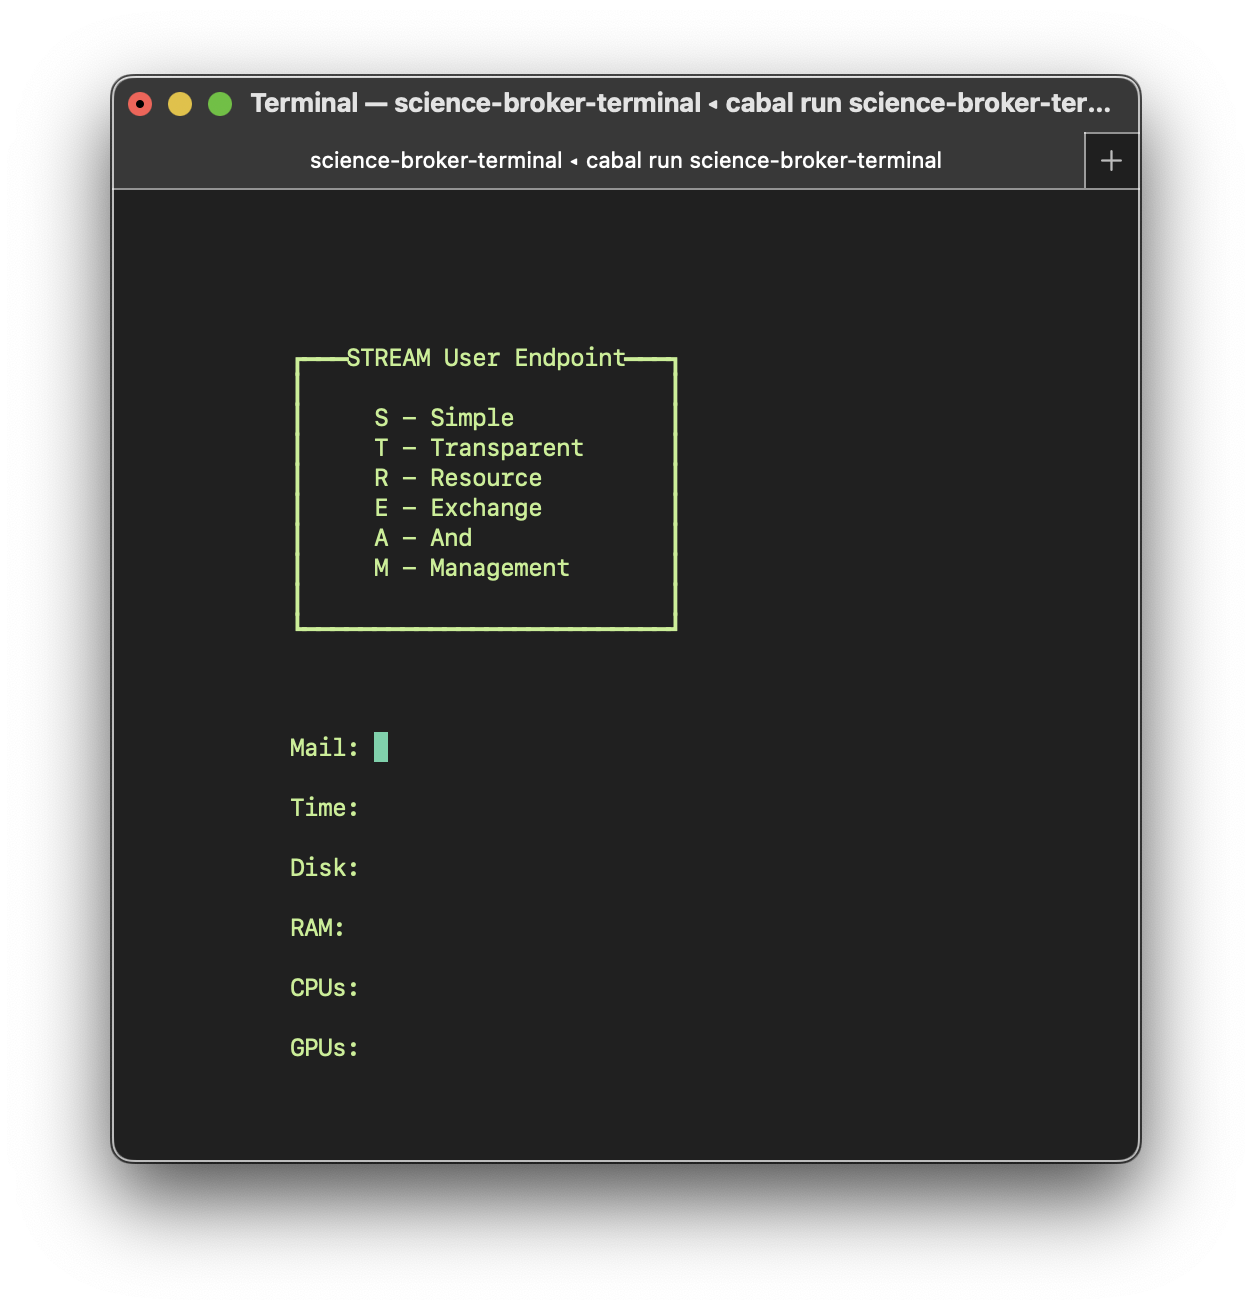
\includegraphics[width=\textwidth]{Frontend-Mockup.png}
\caption{A mock-up of the ``Front-end'' Terminal User Interface.}
\end{figure}


\section{Work Delegation}

\subsection{Main task ``umbrellas'' to be completed:}

\begin{itemize}
\item Backend
\item Frontend
\item Containerization
\item Replication
\end{itemize}

\subsection{Who will do what?}

\begin{itemize}
\item \WorkloadStudentTaksPair{Isa Jafarov}{Backend Broker; centralized job/resource database, job queuing}
\item \WorkloadStudentTaksPair{Nan Jia}{Docker and Kubernetes startup scripts/containerization}
\item \WorkloadStudentTaksPair{Alex Washburn}{TUI \KeyWord{Endpoint}s, scheduling algorithm}
\item \WorkloadStudentTaksPair{Rose Wong}{Backend Backup/Replication}
\end{itemize}


\section{Estimated Timeline}

\begin{center}
\begin{tabular}{ |c| m{9.5cm}| l | c |} 
\hline
Week & Planned Work Items& Deliverable & Date\\
\hline
\MonthDayFormat{04}{16} & System design, GENI research & Project Plan & \MonthDayFormat{04}{23}\\ 
\MonthDayFormat{04}{23} & Frontend TUI, GENI experimentation, containerization & \makebox[6mm][l]{1st} Presentation & \MonthDayFormat{05}{01}\\
\MonthDayFormat{04}{30} & Replication, backups, scheduling algorithm & \makebox[2.85cm]{\hfill---~---\hfill} &  ---~--- \\
\MonthDayFormat{05}{07} & Backend UI, job status feeback, resource utilization  & \makebox[6mm][l]{2nd} Presentation &  \MonthDayFormat{05}{15} \\
\MonthDayFormat{05}{15} & Finalize everything! & Project Report &  \MonthDayFormat{05}{22} \\
\hline
\end{tabular}
\end{center}

\end{document}
